\documentclass[noinstructornotes]{ximera}
%handout:  for handout version with no solutions or instructor notes
%handout,instructornotes:  for instructor version with just problems and notes, no solutions
%noinstructornotes:  shows only problem and solutions

%% handout
%% space
%% newpage
%% numbers
%% nooutcomes

%I added the commands here so that I would't have to keep looking them up
%\newcommand{\RR}{\mathbb R}
%\renewcommand{\d}{\,d}
%\newcommand{\dd}[2][]{\frac{d #1}{d #2}}
%\renewcommand{\l}{\ell}
%\newcommand{\ddx}{\frac{d}{dx}}
%\everymath{\displaystyle}
%\newcommand{\dfn}{\textbf}
%\newcommand{\eval}[1]{\bigg[ #1 \bigg]}

%\begin{image}
%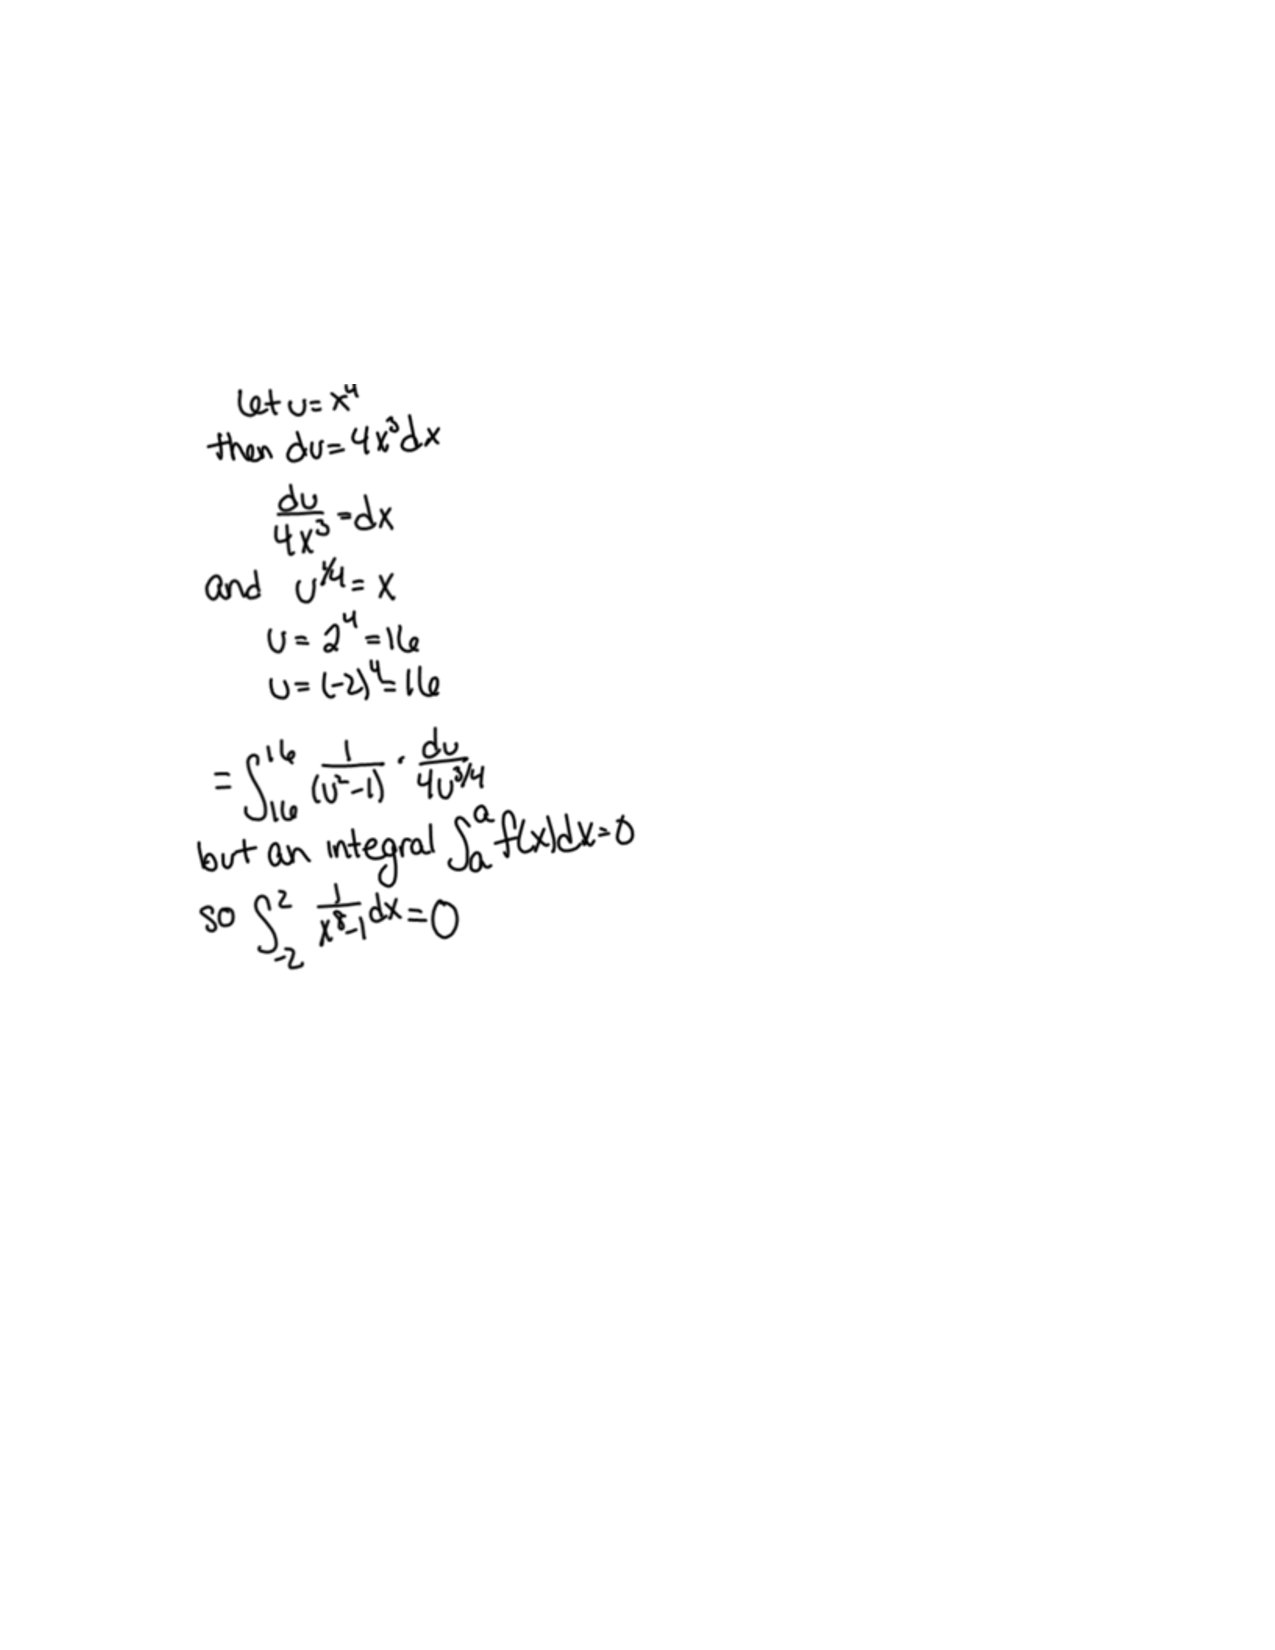
\includegraphics[trim= 170 420 250 180]{Figure1.pdf}
%\end{image}

%add a ``.'' below when used in a specific directory.
\newcommand{\RR}{\mathbb R}
\renewcommand{\d}{\,d}
\newcommand{\dd}[2][]{\frac{d #1}{d #2}}
\renewcommand{\l}{\ell}
\newcommand{\ddx}{\frac{d}{dx}}
\newcommand{\dfn}{\textbf}
\newcommand{\eval}[1]{\bigg[ #1 \bigg]}

\usepackage{multicol}

\renewenvironment{freeResponse}{
\ifhandout\setbox0\vbox\bgroup\else
\begin{trivlist}\item[\hskip \labelsep\bfseries Solution:\hspace{2ex}]
\fi}
{\ifhandout\egroup\else
\end{trivlist}
\fi} %% we can turn off input when making a master document

\title{Basic approaches}  

\begin{document}
\begin{abstract}		\end{abstract}
\maketitle



\begin{comment}
\section{Warm up:}

	\begin{freeResponse}
	
	\end{freeResponse}
	
\begin{instructorNotes}

\end{instructorNotes}
\end{comment}







\section{Group work:}



%problem 1
\begin{problem}
Evaluate
	\[
	\int \frac{5x^3 - 6x + 2}{x-5} \d x.
	\]
	\begin{freeResponse}
	When integrating a rational function (i.e., a fraction of polynomials) where the degree of the numerator is greater than or equal to the degree of the denominator, we need to use long division to simplify the expression.  
	
	\begin{image}
	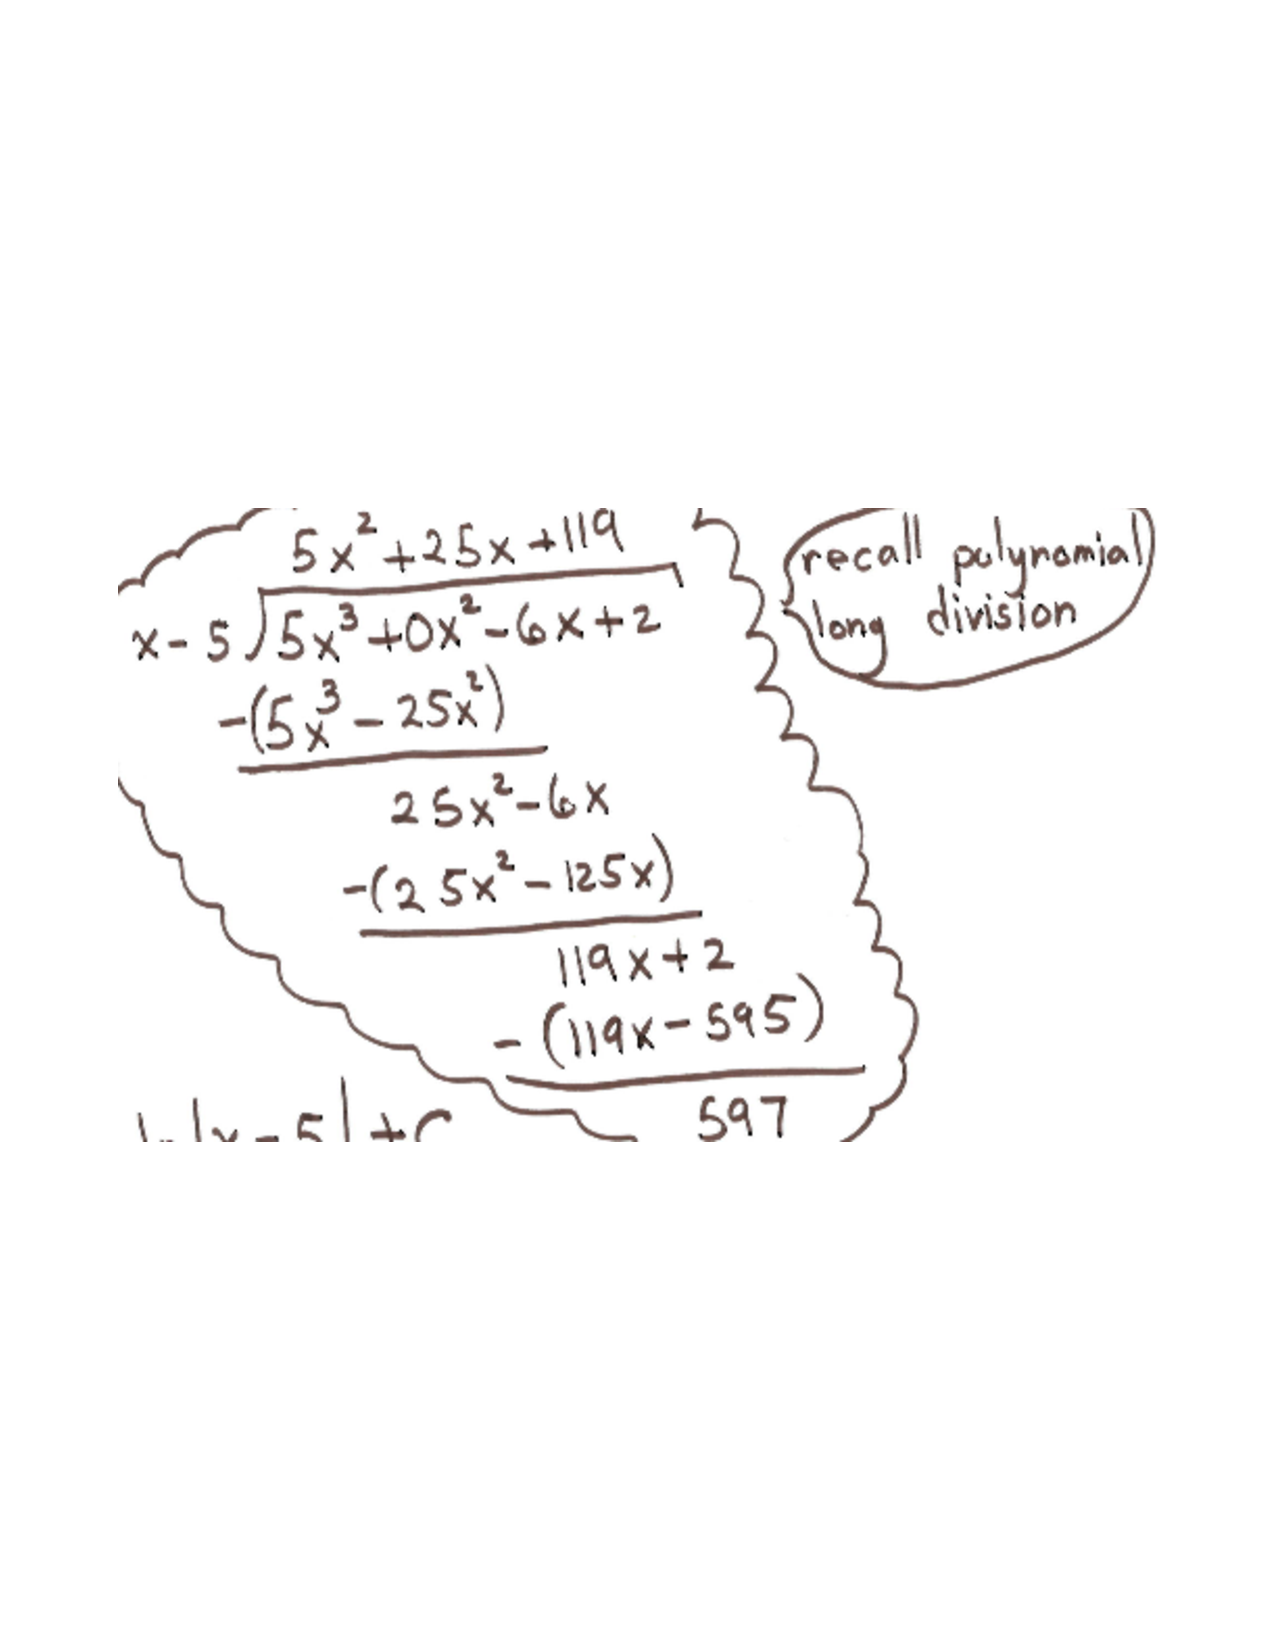
\includegraphics[trim= 170 220 250 250, scale=0.7]{Figure7-1-1.pdf}
	\end{image}
	
	So
		\[
		\frac{5x^3 - 6x + 2}{x-5} = 5x^2 + 25x + 119 + \frac{597}{x-5}
		\]
	and therefore
		\begin{align*}
		\int \frac{5x^3 - 6x + 2}{x-5} \d x &= \int \left( 5x^2 + 25x + 119 + \frac{597}{x-5} \right) \d x  \\
		&= \frac{5}{3} x^3 + \frac{25}{2} x^2 + 119x + 597 \int \frac{1}{x-5} \d x.
		\end{align*}
	To evaluate
		\[
		\int \frac{1}{x-5} \d x
		\]
	we technically should perform a substitution.  
	But since $\ddx (x-5) = 1$, we can treat $x-5$ as a variable during integration.  
	Thus
		\[
		\int \frac{1}{x-5} \d x = \ln |x-5|
		\]
	and therefore
		\[
		\int \frac{5x^3 - 6x + 2}{x-5} \d x = \frac{5}{3} x^3 + \frac{25}{2} x^2 + 119x + 597 \ln |x-5| + C.
		\]
	\end{freeResponse}
	
\end{problem}

\begin{instructorNotes}

\end{instructorNotes}







%problem 2
\begin{problem}
Evaluate
	\[
	\int \frac{5}{3^{2x} + 3^{-2x}} \d x.
	\]
	\begin{freeResponse}
	
	\end{freeResponse}
		
\end{problem}

\begin{instructorNotes}

\end{instructorNotes}







%problem 3
\begin{problem}
Evaluate the following integrals
	\begin{enumerate}
	
	\item  $\int \frac{\cos x}{1 + \sin x} \d x$
	\begin{freeResponse}
	
	\end{freeResponse}
	
	
	
	\item  $ \int \frac{1}{\sin x - 1} \d x$
	\begin{freeResponse}
	
	\end{freeResponse}
	
	\end{enumerate}

\end{problem}

\begin{instructorNotes}

\end{instructorNotes}







%problem 4
\begin{problem}
Evaluate the following integrals
	\begin{enumerate}
	
	\item  $ \frac{13}{\sqrt{12x - x^2 - 20}} \d x$
	\begin{freeResponse}
	
	\end{freeResponse}
	
	
	
	\item  $\int \frac{13x^3}{\sqrt{12x^6 - x^8 - 20x^4}} \d x$
	\begin{freeResponse}
	
	\end{freeResponse}
	
	
	
	\item  $\int \frac{13e^{4x}}{\sqrt{ 12e^{6x} - e^{8x} - 20e^{4x} }} \d x$
	\begin{freeResponse}
	
	\end{freeResponse}
	
	\end{enumerate}

\end{problem}

\begin{instructorNotes}

\end{instructorNotes}
















	
	
	
	
	
	
	
	
	

	










								
				
				
	














\end{document} 


















